\documentclass[a4paper,UKenglish,cleveref, autoref, thm-restate]{lipics-v2021}
%This is a template for producing LIPIcs articles. 
%See lipics-v2021-authors-guidelines.pdf for further information.
%for A4 paper format use option "a4paper", for US-letter use option "letterpaper"
%for british hyphenation rules use option "UKenglish", for american hyphenation rules use option "USenglish"
%for section-numbered lemmas etc., use "numberwithinsect"
%for enabling cleveref support, use "cleveref"
%for enabling autoref support, use "autoref"
%for anonymousing the authors (e.g. for double-blind review), add "anonymous"
%for enabling thm-restate support, use "thm-restate"
%for enabling a two-column layout for the author/affilation part (only applicable for > 6 authors), use "authorcolumns"
%for producing a PDF according the PDF/A standard, add "pdfa"

%\pdfoutput=1 %uncomment to ensure pdflatex processing (mandatatory e.g. to submit to arXiv)
%\hideLIPIcs  %uncomment to remove references to LIPIcs series (logo, DOI, ...), e.g. when preparing a pre-final version to be uploaded to arXiv or another public repository

%\graphicspath{{./graphics/}}%helpful if your graphic files are in another directory

\bibliographystyle{plainurl}% the mandatory bibstyle

\title{A Diagrammatic Calculus for a Functional Model of Natural Language Semantics} %TODO Please add

%\titlerunning{Dummy short title} %TODO optional, please use if title is longer than one line

\author{Matthieu Pierre Boyer}{DI ENS, Paris, France \and Department of Linguistics, Yale University, USA \and \url{http://www.eleves.ens.fr/home/mpboyer}}{matthieu.boyer@ens.fr}{https://orcid.org/0000-0002-1825-0097}{}
\author{Simon Charlow}{Department of Linguistics, Yale University, USA}{simon.charlow@yale.edu}{https://orcid.org/0000-0002-1825-0097}{}

\authorrunning{M. P. Boyer and S. Charlow}

\Copyright{Matthieu P. Boyer and Simon Charlow}

\ccsdesc[100]{Models of computation. Document management and text processing.} %TODO mandatory: Please choose ACM 2012 classifications from https://dl.acm.org/ccs/ccs_flat.cfm 

\keywords{Typing, Natural Language Semantics, Parsing, Side Effects, String Diagrams} %TODO mandatory; please add comma-separated list of keywords

\category{Student Paper} %optional, e.g. invited paper

\relatedversion{} %optional, e.g. full version hosted on arXiv, HAL, or other respository/website
%\relatedversiondetails[linktext={opt. text shown instead of the URL}, cite=DBLP:books/mk/GrayR93]{Classification (e.g. Full Version, Extended Version, Previous Version}{URL to related version} %linktext and cite are optional

%\supplement{Link to a code for the parser will %optional, e.g. related research data, source code, ... hosted on a repository like zenodo, figshare, GitHub, ...
%\supplementdetails[linktext={opt. text shown instead of the URL}, cite=DBLP:books/mk/GrayR93, subcategory={Description, Subcategory}, swhid={Software Heritage Identifier}]{General Classification (e.g. Software, Dataset, Model, ...)}{URL to related version} %linktext, cite, and subcategory are optional

\acknowledgements{I want to thank my mother for the knitting and putting up
  with me peeling potatos to try knitting with toothpicks; Antoine Groudiev
  for his precious insights on how to label equations; Paul-André Melliès for
  his insights; Bob Frank and Bella Senturia for the help with the minimalistic
  merge syntactic theories; and of course, Simon Charlow for his advising
  during my time at Yale, and his help around the linguistics questions that
definitely arose.}

% \nolinenumbers %uncomment to disable line numbering

%Editor-only macros:: begin (do not touch as author)%%%%%%%%%%%%%%%%%%%%%%%%%%%%%%%%%%
\EventEditors{John Q. Open and Joan R. Access}
\EventNoEds{2}
\EventLongTitle{42nd Conference on Very Important Topics (CVIT 2016)}
\EventShortTitle{CVIT 2016}
\EventAcronym{CVIT}
\EventYear{2016}
\EventDate{December 24--27, 2016}
\EventLocation{Little Whinging, United Kingdom}
\EventLogo{}
\SeriesVolume{42}
\ArticleNo{23}
%%%%%%%%%%%%%%%%%%%%%%%%%%%%%%%%%%%%%%%%%%%%%%%%%%%%%%

% Document defined Commands
\usepackage{bigstrut}
\usepackage{makecell}
\usepackage{emoji}
\usepackage{tikz-dependency}
\usepackage{diag}

\def\cont{\Gamma\vdash}
\def\poulpe{\qquad}

\setlength\belowcaptionskip{0pt}
\setlength\abovecaptionskip{\baselineskip}

\DeclareMathOperator{\Var}{Var}

\def\ppl{\mathbin{+\mkern-12mu+}}

\makeatletter
\renewenvironment{thebibliography}[1]
     {\section{\bibname}
      \@mkboth{\MakeUppercase\bibname}{\MakeUppercase\bibname}%
      \list{\@biblabel{\@arabic\c@enumiv}}%
           {\settowidth\labelwidth{\@biblabel{#1}}%
            \leftmargin\labelwidth
            \advance\leftmargin\labelsep
            \@openbib@code
            \usecounter{enumiv}%
            \let\p@enumiv\@empty
            \renewcommand\theenumiv{\@arabic\c@enumiv}}%
      \sloppy
      \clubpenalty4000
      \@clubpenalty \clubpenalty
      \widowpenalty4000%
      \sfcode`\.\@m}
     {\def\@noitemerr
       {\@latex@warning{Empty `thebibliography' environment}}%
      \endlist}

\def\black@or@white#1#2{%
  \@tempdima#2 pt
  \ifdim\@tempdima>0.5 pt
    \definecolor{temp@c}{gray}{0}%
  \else
    \definecolor{temp@c}{gray}{1}%
  \fi}
\def\letterbox#1#{\protect\letterb@x{#1}}
\def\letterb@x#1#2#3{%
  \colorlet{temp@c}[gray]{#2}%
  \extractcolorspec{temp@c}{\color@spec}%
  \expandafter\black@or@white\color@spec
  {\color#1{temp@c}\tallcbox#1{#2}{#3}}}
\def\tallcbox#1#{\protect\color@box{#1}}
\def\color@box#1#2{\color@b@x\relax{\color#1{#2}}}
\long\def\color@b@x#1#2#3%
 {\leavevmode
  \setbox\z@\hbox{{\set@color#3}}%
  \ht\z@\ht\strutbox
  \dp\z@\dp\strutbox
  {#1{#2\color@block{\wd\z@}{\ht\z@}{\dp\z@}\box\z@}}}
\makeatother

\contourlength{0.005em}
\def\backbox#1{\letterbox{Lavender!40}{\contour{black}{#1}}}

\def\ty#1{\backbox{\tt\color{yulm!90!black}#1}}
\def\f#1{\backbox{\tt\color{vulm}#1}}
\def\w#1{\mathbf{#1}\,}

\def\e{\ty{e}}
\def\t{\ty{t}}
\def\r{\ty{r}}

\newcolumntype{C}{>{$}c<{$}}
\newcolumntype{L}{>{$}l<{$}}
\newcolumntype{R}{>{$}r<{$}}
\def\fmap{\texttt{fmap}}


\makeatletter
\newcommand{\@word}[4][]{%
	#2 & #3 & #4\\
\ifx&#1&%
	%
\else
	&\multicolumn{2}{l}{Generalizes to \textbf{#1}}\\%
\fi%
}
\def\word#1#2#3#4{\@word[#4]{#1}{#2}{#3}}
\makeatother

\usepackage{calc}

\makeatletter
\def\textSq#1{%
\begingroup% make boxes and lengths local
\setlength{\fboxsep}{0.4ex}% SET ANY DESIRED PADDING HERE
\setbox1=\hbox{#1}% save the contents
\setlength{\@tempdima}{\maxof{\wd1}{\ht1+\dp1}}% size of the box
\setlength{\@tempdimb}{(\@tempdima-\ht1+\dp1)/2}% vertical raise
\raise-\@tempdimb\hbox{\fbox{\vbox to \@tempdima{%
  \vfil\hbox to \@tempdima{\hfil\copy1\hfil}\vfil}}}%
\endgroup%
}
\def\Sq#1{\textSq{\ensuremath{#1}}}%

\def\c@lsep{2.3}
\def\r@wsep{.8}

\tikzset{
	uptree/.style={
			draw=green!80!black,
			thick,
		},
	typenode/.style={
			align=center,
			text width=24mm,
			%font={\large},
		},
	treenode/.style={
			align=center,
			text width=24mm,
		},
	wordnode/.style={
			inner sep=0pt,
			align=center,
			font={\large},
		},
	downtree/.style={
			draw=red!80!black,
			thick,
		},
}

\newcommand{\wnode}[3]{%
	\node (#2) at (#1*\c@lsep, 0) [wordnode] {#2};
	\node[anchor=north] (#2-) at ($(#1*\c@lsep, 0) + (0, -.142)$) [typenode] {\ensuremath{#3}};
}
\newcommand{\utnode}[3]{%
	\path let \p1 = (#2.north), \p2 = (#3.north) in coordinate (Q1) at (\x1, {max(\y1, \y2)});
	\path let \p1 = (#2.north), \p2 = (#3.north) in coordinate (Q2) at (\x2, {max(\y1, \y2)});
	\node (#2#3) at ($($(Q1)!0.5!(Q2)$) + (0, 1)$) [treenode] {\ensuremath{#1}};
	\draw[uptree] ($(#2.north) + (0, .142)$) -- (#2#3.south);
	\draw[uptree] ($(#3.north) + (0, .142)$) -- (#2#3.south);
}
\newcommand{\dtnode}[4][0.5]{%
	\path let \p1 = (#3.south), \p2 = (#4.south) in coordinate (Q1) at (\x1, {min(\y1, \y2)});
	\path let \p1 = (#3.south), \p2 = (#4.south) in coordinate (Q2) at (\x2, {min(\y1, \y2)});
	\node (#3#4) at ($($(Q1)!#1!(Q2)$) + (0, -1)$) [treenode] {\ensuremath{#2}};
	\draw[downtree] ($(#3.south) + (0, -.142)$) -- (#3#4.north);
	\draw[downtree] ($(#4.south) + (0, -.142)$) -- (#3#4.north);
}

\def\inputtikz#1{
	\ifnum\tikzimp@rt=1
		\input{figures/#1}
	\else
		\ensuremath{\text{\Huge\color{vulm}A TikZ PICTURE GOES HERE.}}
	\fi
}
\makeatother

\catstyle{catone}{gray!50}
\catstyle{catmc}{vulm!10!yulm}
\catstyle{catmca}{vulm!20!yulm}
\catstyle{catmcb}{vulm!30!yulm}
\catstyle{catmcc}{vulm!40!yulm}
\catstyle{catmcd}{vulm!50!yulm}
\catstyle{catmce}{vulm!60!yulm}
\catstyle{catmcf}{vulm!70!yulm}
\catstyle{catmcg}{vulm!80!yulm}
\catstyle{catmch}{vulm!90!yulm}

\def\din#1{#1\mathrm{.S}}
\def\dnb#1{#1\mathrm{.N}}
\def\dlb#1#2{#1\mathrm{.L}\left(#2\right)}
\def\dl#1{#1\mathrm{.L}}
\def\dnlg#1{#1\mathrm{.h}}
\def\dnin#1{#1\mathrm{.in}}
\def\dnout#1{#1\mathrm{.out}}

\newcounter{lingexcnt}
\newcounter{tmplingexcnt}
\renewcommand*{\thelingexcnt}{(\arabic{lingexcnt})}
\newenvironment{sentence}[1][]{
     \begin{list}{\thelingexcnt}{\refstepcounter{lingexcnt}}\item
     \ifnum\pdfstrcmp{#1}{}=0\else\label{#1}\fi
}{\end{list}}

\newenvironment{nsentence}{%
     \setcounter{tmplingexcnt}{\value{lingexcnt}}
     \addtocounter{tmplingexcnt}{-1}
     \begin{list}{\thelingexcnt}{
         \usecounter{lingexcnt}
         \setcounter{lingexcnt}{\value{tmplingexcnt}}
         \refstepcounter{lingexcnt}
     }
}{\end{list}}

\newcommand*{\oneSentence}[2][]{\begin{sentence}[#1]#2\end{sentence}}


\begin{document}

\maketitle

\begin{abstract}
	In this paper, we study a functional programming approach to natural language
	semantics, allowing us to increase the expressivity of a more traditional
	denotation style.
	We will formalize a category based type and effect system, and construct a
	diagrammatic calculus to model parsing and handling of effects, and use it to
	efficiently compute the denotations for sentences.
\end{abstract}

\section{Introduction}
What is \emph{a chair}? How do I know that \emph{Jupiter, a planet}, is
\emph{a planet}?
To answer those questions, \cite{bumfordEffectdrivenInterpretationFunctors2025}
provide a \textsc{Haskell} based view on the notion of typing in natural
language semantics.
Their main idea is to include a layer of effects which allows for improvements
in the expressiveness of the denotations used.
This allows to model complex concepts such as anaphoras, or non-determinism in
an easy way, independent of the actual way the words are represented.
Indeed, when considering the usual denotations of words as typed lambda-terms,
this allows us to solve the issue of meaning getting lost through impossible
typing, while still being able to compose meanings properly.
When two expressions have the same syntactic distribution, they must also have
the same type, which forces quantificational noun phrases to have the same type
as proper nouns: the entity type $\e$.
However, there is no singular entity that is the referent of \emph{every
	planet}, and so, the type system gets in the way of meaning, instead of being
a tool at its service.

\smallskip

Our formalism is inscribed in the contemporary natural language semantic
theories which are based on three main elements: a \emph{lexicon}, a
\emph{syntactic description} of the language, and a theory of
\emph{composition}.
More specifically, we explain how to extend the domain of the lexicon and the
theory of composition to account for the phenomena described above.
We will not be discussing most of the linguistic foundations for the usage of
the formalism, nor its usefulness.
We refer the reader to \cite{bumfordEffectdrivenInterpretationFunctors2025} to
get an overview of the linguistic considerations that are the base of the
theory.

\smallskip

In this paper, we will provide a formal definition of an enhanced type and
effect system for natural language semantics, based on categorical tools.
This will increase the complexity (both in terms of algorithmic operations and
in comprehension of the model) of the parsing algorithms, but through the use
of string diagrams to model the effect of composition on potential effectful
denotations (or more generally computations), we will provide efficient
algorithms for computing the set of meanings of a sentence, from the meaning of
its components.

\section{Related Work}
This is not the first time a categorical representation of compositional
semantics of natural language is proposed,
\cite{coeckeMathematicalFoundationsCompositional2010} already suggested an
approach based on monoidal categories using an external model of meaning.
What our approach gives more, is additional latitude for the definition of
denotations in the lexicon, and a visual explanation of the difference between
multiple possible parsing trees.
We will go back later on the differences between their Lambek inspired grammars
and our more abstract way of looking at the semantic parsing of a sentence.

\smallskip

On a completely different approach,
\cite{marcollimatildeetchomskynoametberwickrobertc.MathematicalStructureSyntactic}
provide a categorical structure based on Hopf algebra and coloured operads
to explain their model of syntax, leading to results at the interface of syntax
and morphology presented in \cite{senturiaAlgebraicStructureMorphosyntax2025}.
Similarly, \cite{melliesCategoricalContoursChomskySchutzenberger2025} provides
a modeling of CFGs using coloured operads.
Our approach is based on the suggestion that merge in syntax can be done using
labels, independent on how it is mathematically modelled.

\section{Categorical Semantics of Effects: A Typing System}
\label{sec:typingsystem}
In this section, we will formalize a type system underlying the theory proposed
in \cite{bumfordEffectdrivenInterpretationFunctors2025}.
To do so, we will designate by $\mL$ our language, as a set of words
(with their associated meaning/denotation) and syntactic rules underlying
the semantic combination.
The absence of syntactic rules is allowed, although it partly defeats the
purpose of this work.
This might be useful when proposing compositional models of learned
representations.

Let $\O\left( \mL \right)$ be the set of words in the language whose semantic
representation is a low-order function and $\mF\left( \mL \right)$ the set of
words whose semantic representation is a functor or high-order function.
Our goals here are to describe more formally, using a categorical vocabulary,
the environment in which the typing system for our language will exist, and how
we connect words and other linguistic objects to the categorical formulation.

\subsection{Typing Category}
\subsubsection{Types}
Let $\mC$ be a closed cartesian category, which is used to represent the
domain of types for our domain of uneffectful denotations.
This represents our main typing system, consisting of types for words $\O(\mL)$
that can be expressed without effects (see Figure \ref{fig:lexicon} for an
example).
Remember that $\mC$ contains a terminal object $\bot$ representing the empty
type or the lack thereof.
We consider as our typing category $\bar{\mC}$ the categorical closure for
exponentials and products of $\mF\left( \mL \right)^{*}\left(\mC\right)$,
which consists of all the different type constructors (ergo, functors) that
could be formed in the language.
In that setting our types are those that can be attained in a finite number
from a finite number of functorial applications from an object of $\mC$.

Formally, we consider for our types the quotient set
$\star = \mathrm{Obj}\left( \bar{\mC} \right)/\mF\left( \mL \right)$.
Since $\mF\left( \mL \right)$ does not induce an equivalence relation on
$\Obj\left( \bar{\mC} \right)$ but a preorder, we consider the chains obtained
by the closure of the relation $x\succeq y \Leftrightarrow \exists F, y = F(x)$
(which should be seen as a subtyping relation as proposed in
\cite{melliesFunctorsAreType2015}).
We also define $\star_{0}$ to be the set obtained when considering types which
have not yet been \emph{affected}, that is $\Obj(\mC)$.
In contexts of polymorphism, we identify $\star_{0}$ to the adequate subset of
$\star$.
In this paradigm, constant objects (or results of fully done computations) are
functions with type $\bot \to \tau$ which we will denote directly by
$\tau \in \star_{0}$.
This will be useful when defining base combinators in Section \ref{sec:parsing}.

\subsubsection{Functors, Applicatives and Monads}
Our point of view has us consider \emph{language functors}\footnote{The
	elements of our language, not the categorical construct.} as polymorphic
functions: for a (possibly restrained) set of base types $S$, a functor is a
function:
\begin{equation*}
	x: \tau\in S\subseteq \star \mapsto F x: F\tau
\end{equation*}
This means that if a functor can be applied to a type, it can also be applied
to all \emph{affected} versions of that type, i.e.
$\mF\left( L \right)(\tau\in \star)$.
This gives us two typing judgements for the functor $F$:
\begin{equation*}
	\frac{\Gamma\vdash x: \tau \in \star_{0}}{\Gamma\vdash F x: F\tau \notin
		\star_{0}} \hspace{2cm} \frac{\Gamma\vdash x:
		\tau}{\Gamma\vdash Fx : F\tau\preceq \tau}
\end{equation*}
We use the same notation for the \emph{language functor} and the
\emph{type functor} in the examples, but it is important to note those are two
different objects, although connected.
More precisely, the \emph{language functor} is to be seen as a function whose
computation yields an effect, while the \emph{type functor} is the endofunctor
of $\bar{\mC}$ (so a functor from $\mC$) that represents the effect in our
typing category.
Examples are provided in Figure \ref{fig:functors}.

\smallskip

In this regard, applicatives and monads only provide with more flexibility on
the ways to combine functions:
they provide intermediate judgements to help with the combination of trees.
For example, the multiplication of the monad provides a new
\emph{type conversion} judgement:
\begin{equation*}
	\frac{\Gamma\vdash x: MM\tau}{\Gamma\vdash x: M\tau \succeq MM\tau}
\end{equation*}
This is actually a special case of the natural transformation rule that we
define below, which means that, in a way, types $MM\star$ and $M\star$ are
equivalent, as there is a canonical way to go from one type to another.
Remember however that $M\star$ is still a proper subtype of $MM\star$ and that
the objects are not actually equal: they are simply equivalent.

\subsubsection{Natural Transformations}
\label{subsubsec:transnat}
We could add judgements directly for adjunctions, but we instead add judgements
for natural transformations, as adjunctions are natural transformations which
arise from \emph{natural} settings.
While in general we do not want to find natural transformations, we want to be
able to express these in three situations:
\begin{enumerate}
	\item Adjunctions.
	\item To deal with the resolution of effects as explained in Section
	      \ref{sec:nondet}
	\item To create \emph{higher-order} constructs which transform words from our
	      language into other words, while keeping the functorial aspect.
	      This idea is developed in Section \ref{par:higherorder}.
\end{enumerate}
To see why we want this rule, which is a larger version of the monad
multiplication and the monad/applicative unit, it suffices to see that the
diagram defining the properties of a natural transformation provides a way
to construct the \emph{correct function} on the \emph{correct functor} side of
types.

\smallskip

In the Haskell programming language, any polymorphic function is
a natural transformation from the first type constructor to the second type
constructor, as proved in \cite{wadlerTheoremsFree1989}.
This will guarantee for us that given a \emph{Haskell} construction for a
polymorphic function, we will get the associated natural transformation.

\paragraph{Handlers}
As introduced by \cite{marsikAlgebraicEffectsHandlers}, the use of handlers
as annotations to the semantic tree of the sentence is an appropriate
formalism.
As considered by \cite{wuEffectHandlersScope2014}, handlers are to be seen
as natural transformations describing the free monad on an algebraic effect.
Considering handlers as so, allows us to directly handle our computations
inside our typing system, by ``transporting'' our functors one order higher up
without loss of information or generality since all our functors undergo the
same transformation.
Using the framework proposed in \cite{vandenbergFrameworkHigherorderEffects2024}
we simply need to create handlers for our effects/functors and we will then
have in our language the result needed.
The only thing we will require from an algebraic handler $h$ is that for any
applicative functor of unit $\eta$, $h\circ \eta = \id$.

\smallskip

Note that the choice of the handler being part of the lexicon or the parser
over the other is a philosophical question more than a semantical one, as both
options will result in semantically equivalent models, the only difference will
be in the way we consider the resolution of effects.
This choice does not arise in the case of the adjunction-induced
handlers.
Indeed here, the choice is caused by the non-uniqueness of the choices for
the handlers as two different speakers may have different ways to resolve the
non-determinism effect that arises from the phrase \textsl{A chair}.
This is the difference with the adjunctions: adjunctions are intrinsic
properties of the coexistence of the effects, while the handlers
are user-defined.

\paragraph{Higher-Order Constructs}
\label{par:higherorder}
Functors may also be used to add plurals, superlatives, tenses, aspects and
other similar constructs which act as function modifiers.
For each of these, we give a functor $\Pi$ corresponding to a new class of
types along with natural transformations for all other functors $F$ which
allows to propagate down the high-order effect.
This transformation will need to be from $\Pi \circ F$ to
$\Pi \circ F \circ \Pi$ or simply $\Pi \circ F \Rightarrow F \circ \Pi$
depending on the situation.
This allows us to add complexity not in the compositional aspects but
in the lexicon aspects, by simply saying that those constructs are predicate
modifiers passed down (with or without side effects) to the arguments of
predicates:
\begin{equation*}
	\begin{aligned}
		\mathbf{future\left( be \right)\left( arg_{1}, arg_{2} \right)}
		 & \xrightarrow{\eta} \mathbf{future\left( be \right)\left( arg_{2} \right)\left( future\left( arg_{1} \right) \right)}                           \\
		 & \xrightarrow{\eta} \mathbf{future \left( be \right) \left( future \left( arg_{2} \right) \right) \left( future \left( arg_{1} \right) \right)}
	\end{aligned}
\end{equation*}

Among other higher-order constructs that might be represented using effects are
scope islands, which could be modelled by a functor that cannot be
passed as argument to words that would otherwise need a closure to be applied
first.
See Figure \ref{fig:tree-rain} for an example, based on theory presented in
\cite{bumfordEffectdrivenInterpretationFunctors2025}, Section 5.4.

\paragraph{Monad Transformers}
In \cite{bumfordEffectdrivenInterpretationFunctors2025}, the authors present
constructions which they call monad transformers or \emph{higher-order
	constructors} and which take a monad as input and return a monad as output.
One way to type those easily would be to simply create, for each such
construct, a monad (the result of the application to any other monad) and a
natural transformation which mimics the application and can be seen as the
constructor.

\subsection{Typing Judgements}\label{subsec:judgements}
To complete this section, Figure \ref{tab:judgements} gives a simple list of different typing composition judgements through which we also re-derzive the subtyping judgement to allow for its implementation.
\begin{figure}
	\begin{align*}
	\forall F \in \mF\left( \mL \right),\poulpe
	\frac{\cont x: \tau \poulpe \cont F: S\subseteq \star \poulpe \overbrace{\tau \in S}^{\exists \tau'\in S, \tau \preceq \tau'}}{\cont Fx: F\tau \preceq \tau}\fracnotate{Cons} \\[.25cm]
	\frac{\cont x: \tau \poulpe \tau \in \star_{0}}{\cont Fx: F\tau \notin \star_{0}}\fracnotate{$FT_{0}$}                                                                        \\[.25cm]
	\frac{\cont x: F\tau_{1} \poulpe \cont \phi: \tau_{1} \to \tau_{2}}{\cont \phi x: F\tau_{2} }\fracnotate{\texttt{fmap}}                                                       \\[.25cm]
	\frac{\cont x: \tau_{1} \poulpe \cont \phi: \tau_{1} \to \tau_{2}}{\cont \phi x: \tau_{2}}\fracnotate{App}                                                                    \\[.5cm]
	\frac{\cont x: A\tau_{1} \poulpe \cont \phi: A\left( \tau_{1} \to \tau_{2} \right)}{\cont \phi x: A\tau_{2}}\fracnotate{\texttt{<*>}}                                         \\[.25cm]
	\frac{\cont x: \tau}{\cont x: A\tau}\fracnotate{\texttt{pure/return}}                                                                                                         \\[.5cm]
	\frac{\cont x: MM\tau}{\cont x: M\tau}\fracnotate{\texttt{>>=}}                                                                                                               \\[.25cm]
	\forall F \overset{\theta}{\Longrightarrow} G,\poulpe \frac{\cont x: F\tau \poulpe \cont G: S' \subseteq \star \poulpe \tau \in S'}{\cont x : G\tau}\fracnotate{\texttt{nat}}
\end{align*}

	\caption{Typing and subtyping judgements for implementation of effects in the
		type system.}
	\label{tab:judgements}
\end{figure}
Note that here, the syntax is not taken into account: a function is always written left of its arguments, whether or not they are actually in that order in the sentence.

\smallskip

Using these typing rules for our semantic parsing steps, it is important to
see that our grammar will still bear ambiguity.
The next sections will explain how to reduce this ambiguity in short enough
time.

Moreover, our current typing system is not decidable, because of the
\texttt{nat/pure/return} rules which may allow for unbounded derivations.
This is not actually an issue because of considerations on handling, as
semantically void units will get removed at that time.
This leads to derivations of sentences to be of bounded height, linear in the
length of the sentence.


\section{Handling Ambiguity}
\label{sec:nondet}
The typing judgements proposed in Section \ref{subsec:judgements} lead to
ambiguity.
In this section we propose ways to get our derivations to a certain normal
form, by deriving an equivalence relation on our derivation and parsing trees,
based on string diagrams.

\subsection{String Diagram Modelisation of Sentences}
\label{subsec:sd}
String diagrams are the Poincaré duals of the usual categorical diagrams when
considered in the $2$-category of categories and functors.
This means that we represent categories as regions of the plane, functors as
lines separating regions and natural transformations as the intersection points
between two lines.

We will always consider application as applying to the right of the line so
that composition is written in the same way as in equations.
This gives us a new graphical formalism to represent our effects using a few
equality rules between diagrams.
The commutative aspect of functional diagrams is now replaced by an equality of
string diagrams, which will be detailed in the following section.

We get a way to visually see the meaning get reduced from effectful composition
to propositional values, without the need to specify what the handler does.
This delimits our usage of string diagrams as ways to look at computations and
a tool to provide equality rules to reduce ambiguity.

\begin{wrapfigure}{r}{.45\textwidth}
	\centering
		\begin{tikzpicture}
		\path coordinate[dot, label=right:$\w{the}$] (the) + (0, 1) coordinate[dot, label=left:$\w{sleeps}$] (sleeps) + (0, 2) coordinate[label=above:$\t$] (bool)
		++(-2, 1) coordinate (ctlthe) + (0, 1) coordinate[label=above:$\f{M}$] (effthe)
		++(2, -2) coordinate[dot, label=left:$\w{cat}$] (cat) + (0, -2) coordinate[label=below:$\bot$] (bot);
		\draw (cat) -- (the) -- (sleeps) -- (bool);
		\draw[name path=effect] (the) to[out=180, in=-90] (ctlthe) -- (effthe);
		\draw[dashed] (bot) -- (cat);
		\begin{pgfonlayer}{background}
			\fill[catone] (bot) rectangle ($(bool) + (1, 0)$);
			\fill[catmca] (bot) rectangle ($(effthe) + (-1, 0)$);
			\fill[catmc] (the) to [out=180, in=-90] (ctlthe) -- (effthe) -- (bool) -- (the);
		\end{pgfonlayer}
	\end{tikzpicture}

\end{wrapfigure}
Let us define the category $\mathds{1}$ with exactly one object and one arrow:
the identity on that object. It will be shown in grey in the string diagrams
below.
A functor of type $\mathds{1} \to \mC$ is equivalent to choosing an object in
$\mC$, and a natural transformation between two such functors $\tau_{1},
	\tau_{2}$ is exactly an arrow in $\mC$ of type $\tau_{1} \to \tau_{2}$.
Knowing that allows us to represent the type resulting from a sequence of
computations as a sequence of strings whose farthest right represents an object
in $\mC$, that is, a base type.

The question of providing rules to compose the string diagrams for parts of the
sentences will be discussed in the next section, as it is related to parsing.

\smallskip

In the end, we will have the need to go from a certain set of strings (the effects that applied) to a single one, through a sequence of handlers, monadic and comonadic rules and so on.
Notice that we never reference the zero-cells and that in particular their colors are purely an artistical touch.

\subsection{Achieving Normal Forms}
\label{subsec:normalforms}
We will now provide a set of rewriting rules on string diagrams (written as
equations) which define the set of different possible reductions.

First, Theorem \ref{thm:isotopy} reminds the main result by \cite{joyalGeometryTensorCalculus1991} about string diagrams which shows that our artistic representation of diagrams is correct and does not modify the equation or the rule we are presenting.
\begin{theorem}[Theorem 1.2 \cite{joyalGeometryTensorCalculus1991}]
	\label{thm:isotopy}
	A well-formed equation between morphism terms in the language of monoidal categories follows from the axioms of monoidal categories if and only if it holds, up to planar isotopy, in the graphical language.
\end{theorem}

Secondly, let us now look at a few of the equations that arise from the
commutation of certain class of diagrams:
\begin{description}
	\item[The \emph{Snake} Equations] are a rewriting of the categorical diagrams
	      which are the defining properties of an adjunction.
	\item[The \emph{(co-)Monadic} Equations] are the string diagrammatic
	      translation of the properties of unitality and associativity of the
	      monad.
	      Similarly, there are co-monadic equations which are the categorical dual
	      of the previous equations.
\end{description}
This set of equations, when added to our reduction rules from the Section
\ref{sec:parsing} explain all the different reductions that can be made to
limit non-determinism in our parsing strategies.
Indeed, considering the equivalence relation $\mathcal{R}$ freely generated
from the equations defined above and the equivalence relationship
$\mathcal{R}'$ of planar isotopy from Theorem \ref{thm:isotopy}, we get a set
of normal forms $\mathcal{N}$ from the set of all well-formed parsing diagrams
$\mD$ defined by:
$\mathcal{N} = \left( \mD / \mathcal{R} \right) / \mathcal{R}'$


\subsection{Computing Normal Forms}
Now that we have a set of rules telling us what we can and cannot do in our model while preserving the equality of the diagrams, we provide a combinatorial description of our diagrams to help compute the possible equalities between multiple reductions of a sentence meaning.

\cite{delpeuchNormalizationPlanarString2022} proposed a combinatorial description to check
in linear time for equality under Theorem \ref{thm:isotopy}.
However, this model does not suffice to account for all of our equations, especially as
labelling will influence the equations for monads, comonads and adjunctions.
To provide with more flexibility (in exchange for a bit of time complexity) we use the
description provided and change the description of inputs and outputs of each $2$-cell by
adding types and enforcing types.
In this section we formally describe the data structure we propose, as well as algorithms for
validity of diagrams and a system of rewriting that allows us to compute the normal forms
for our system of effects.

\subsubsection{Representing String Diagrams}
We follow \cite{delpeuchNormalizationPlanarString2022} in their combinatorial description
of string diagrams. We describe a diagram by an ordered set of its $2$-cells (the natural
transformations) along with the number of input strings, for each $2$-cell the following
information:
\begin{itemize}
	\item Its horizontal position: the number of strings that are right of it.
	\item Its type: an array of effects that are the inputs to the natural
	      transformation and an array of effects that are the outputs to the
	      natural transformation.
\end{itemize}
We will then write a diagram $D$ as a tuple of $3$ elements:
$\left( D.N, D.S, D.L \right)$ where $D.N$ is a positive integers representing the
height (or number of nodes) of $D$, $D.S$ is an array for the input strings of $D$ and
where $D.L$ is a function which takes a natural number smaller than $D.N - 1$ and
returns its type as a tuple of arrays
$nat = \left( \dnlg{nat}, \dnin{nat}, \dnout{nat} \right)$.
From this, we can derive a naive algorithm to check if a string diagram is
valid or not.

\smallskip

Since our representation contains strictly more information (without slowing
access by a non-constant factor) than the one it is based on, our
datastructure supports the linear and polynomial time algorithms proposed with
the structure by \cite{delpeuchNormalizationPlanarString2022}.
In particular our structure can be normalized in time
$\O\left( n \times \sup_{i} \abs{\dnin{\dlb{D}{i}}} + \abs{\dnout{\dlb{D}{i}}}
	\right)$, which depends on our lexicon but most of the times will be linear
time.

\subsubsection{Equational Reductions}
We are faced a problem when computing reductions using the equations for our diagrams
which is that by definition, an equation is symmetric.
To solve this issue, we only use equations from left to right to reduce as much as
possible our result instead.
This also means that trivially our reduction system computes normal forms: it suffices
to re-apply the algorithm for recumbent equivalence after the rest of equational
reduction is done.
Moreover, note that all our reductions are either incompatible or commutative, which
leads to a confluent reduction system, and the well definition of our normal forms:
\begin{theorem}[Confluence]\label{thm:confluence}
	Our reduction system is confluent and therefore defines normal forms:
	\begin{enumerate}
		\item Right reductions are confluent and therefore define \emph{right} normal forms for
		      diagrams under the equivalence relation induced by exchange.
		\item Equational reductions are confluent and therefore define \emph{equational}
		      normal forms for diagrams under the equivalence relation induced by exchange.
	\end{enumerate}
\end{theorem}

Before proving the theorem, let us first provide the reductions for the different
equations for our description of string diagrams.
\begin{description}
	\item[The Snake Equations]
	      First, let's see when we can apply the equation for $\id_{L}$ to a
	      diagram $D$ which is in \emph{right} normal form, meaning it's been
	      right reduced as much as possible.
	      Suppose we have an adjunction $L \dashv R$.
	      Then we can reduce $D$ along the equation at $i$ if, and only if:
	      \begin{itemize}
		      \item $\dnlg{\dlb{D}{i}} = \dnlg{\dlb{D}{i + 1}} - 1$
		      \item $\dlb{D}{i} = \eta_{L, R}$
		      \item $\dlb{D}{i + 1} = \epsilon_{L, R}$
	      \end{itemize}
	      This comes from the fact that we can't send either $\epsilon$
	      above $\eta$ using right reductions and
	      that there cannot be any natural transformations between the two.
	      Obviously the equation for $\id_{R}$ works the same.
	      Then, the reduction is easy: we simply delete both strings,
	      removing $i$ and $i + 1$ from $D$ and reindexing the other nodes.
	\item[The Monadic Equations] For the monadic equations, we only use
	      the unitality equation as a way to reduce the number of natural
	      transformations, since the goal here is to attain normal forms
	      and not find all possible reductions.
	      We ask that associativity is always used in the direct
	      sense $\mu\left( \mu\left( TT \right),T \right) \to \mu\left(
		      T\mu\left( TT \right) \right)$ so that the algorithm terminates.
	      We use the same convention for the comonadic equations.
	      The validity conditions are as easy to define for the monadic
	      equations as for the \emph{snake} equations when considering
	      diagrams in \emph{right} normal forms.
	      Then, for unitality we simply delete the nodes
	      and for associativity we switch the horizontal
	      positions for $i$ and $i + 1$.
\end{description}

\begin{proof}[Proof of the Confluence Theorem]
	The first point of this theorem is exactly Theorem 4.2
	in \cite{delpeuchNormalizationPlanarString2022}.
	To prove the second part, note that the reduction process terminates as
	we strictly decrease the number of $2$-cells with each reduction.
	Moreover, our claim that the reduction process is confluent is obvious
	from the associativity equation and the fact the other
	equations delete nodes.
	Since right reductions do not modify the equational reductions, and thus
	right reducing an equational normal form yields an equational normal form,
	combining the two systems is done without issue, completing our proof of
	Theorem \ref{thm:confluence}.
\end{proof}

\begin{theorem}[Normalization Complexity]
	\label{thm:normalize}
	Reducing a diagram to its normal form is done in polynomial time in
	the number of natural transformations in it.
\end{theorem}
\begin{proof}
	Let's now give an upper bound on the number of reductions.
	Since each reductions either reduces the number of $2$-cells or applies the
	associativity of a monad, we know the number of reductions is linear in the
	number of natural transformations.
	Moreover, since checking if a reduction is possible at height $i$ is done in
	constant time, checking if a reduction is possible at a step is done in
	linear time, rendering the reduction algorithm quadratic in the number of
	natural transformations.
	Since we need to \emph{right} normalize before and after this method, and
	that this is done in linear time, our theorem is proved.
\end{proof}



\section{Efficient Semantic Parsing}
\label{sec:parsing}
In this section we explain our algorithms and heuristics for efficient semantic
parsing with as little non-determinism as possible, and reducing time complexity
of our parsing strategies.

\subsection{Syntactic-Semantic Parsing}
Using a naïve strategy to compute judgements from the trees yields an
exponential algorithm, the best way to improve the algorithm, is to directly
leave the naïve strategy.
To do so, we could simply extend the grammar system used to do the syntactic
part of the parsing.
In this section, we will take the example of a CFG since it suffices to create
our typing combinators,
In Figure \ref{fig:combination-cfg}, we explicit a grammar of combination
modes, based on \cite{bumfordEffectdrivenInterpretationFunctors2025} as it
simplifies the rewriting of our typing judgements in a CFG.

\begin{figure}
	\centering
	{\centering
\setlength{\columnsep}{-1.5cm}
\begin{multicols}{2}
	\def\arraystretch{1.2}
	\begin{mgrammar}
		\gskip
		\firstrule{>, b}{\left(a\to b\right), a}{}
		\firstrule{<, b}{a, \left(a \to b\right)}{}
		\firstrule{\wedge, a \to \t}{\left(a \to \t\right), \left(a \to \t\right)}{}
		\firstrule{\vee, a \to \t}{\left(a \to \t\right), \left(a \to \t\right)}{}
		\gskip
		\firstrule{\combJ_{\f{F}}\  \f{F}\tau}{\f{F}\f{F}\tau}{}
		\lfrule{\combDN_{\f{C}}\  \tau}{\f{C}_{\tau}\tau}{}
	\end{mgrammar}

	\def\arraystretch{1.3}
	\begin{mgrammar}
		\firstrule{\combML_{\f{F}} \left(\alpha, \beta\right)}{\f{F}\alpha, \beta}{}
		\firstrule{\combMR_{\f{F}} \left(\alpha, \beta\right)}{\alpha, \f{F}\beta}{}
		\firstrule{\combA_{\f{F}} \left(\alpha, \beta\right)}{\f{F}\alpha, \f{F}\beta}{}
		\firstrule{\combUR_{\f{F}} \left(\alpha \to \alpha', \beta\right)}{\f{F}\alpha\to \alpha', \beta}{}
		\firstrule{\combUL_{\f{F}} \left(\alpha, \beta\to \beta'\right)}{\alpha, \f{F}\beta \to \beta'}{}
		\firstrule{\combC_{\f{L}\f{R}} \left(\f{L} \alpha, \f{R}\beta\right)}{\left(\alpha, \beta\right)}{}
		\firstrule{\combER_{\f{R}} \left(\f{R}\left(\alpha \to \alpha'\right), \beta\right)}{\alpha\to \f{R}\alpha', \beta}{}
		\lfrule{\combEL_{\f{R}} \left(\alpha, \f{R}\left(\beta \to \beta'\right)\right)}{\alpha, \beta\to \f{R}\beta'}{}
	\end{mgrammar}
\end{multicols}
}

	\caption{Possible type combinations in the form of a near CFG}
	\label{fig:combination-cfg}
\end{figure}

This grammar works in five major sections:
\begin{enumerate}
	\item We reintroduce the grammar defining the type and effect system.
	\item We introduce a structure for the semantic parse trees and their labels,
	      the combination modes from
	      \cite{bumfordEffectdrivenInterpretationFunctors2025}.
	\item We introduce rules for basic type combinations.
	\item We introduce rules for higher-order unary type combinators.
	\item We introduce rules for higher-order binary type combinators.
\end{enumerate}

\begin{figure}[H]
	\centering
	\def\arraystretch{1.5}
% f · x = (\fmap_{\f{F}} f) (x)
% \eta = pure 
\begin{multicols}{2}
	$	>                    = \lambda \phi. \lambda x. \phi x $\\[1.5ex]
	$ <                    = \lambda x. \lambda \phi. \phi x $\\[1.5ex]
	$ \combML_{\f{F}}      = \lambda M. \lambda x. \lambda y. (\fmap_{\f{F}} \lambda a. M(a, y)) x $\\[1.5ex]
	$ \combMR_{\f{F}}      = \lambda M. \lambda x. \lambda y. (\fmap_{\f{F}} \lambda b. M(x, b)) y $\\[1.5ex]
	$	\combA_{\f{F}}       = \lambda M. \lambda x. \lambda y. (\fmap_{\f{F}}\lambda a. \lambda b. M(a, b))(x) \texttt{<*>} y $\\[1.5ex]
	$	\combUL_{\f{F}}      = \lambda M. \lambda x. \lambda \phi. M(x, \lambda b. \phi(\eta_{\f{F}} b))$\\[1.5ex]
	$	\combUR_{\f{F}}      = \lambda M. \lambda \phi. \lambda y. M(\lambda a. \phi(\eta_{\f{F}} a),y) $\\[1.5ex]
	$ \combJ_{\f{F}}       = \lambda M. \lambda x. \lambda y. \mu_{\f{F}} M(x, y) $\\[1.5ex]
	$	\combC_{\f{L}\f{R}}  = \lambda M. \lambda x. \lambda y. \epsilon_{\f{L}\f{R}}(\fmap_{\f{L}}(\lambda l. \fmap_{\f{R}}(\lambda r. M(l, r))(y)) (x)) $\\[1.5ex]
	$	\combEL_{\f{R}}      = \lambda M. \lambda \phi. \lambda y. M(\Upsilon_{\f{R}} \phi, y)$\\[1.5ex]
	$	\combER_{\f{R}}      = \lambda M. \lambda x. \lambda \phi. M(x, \Upsilon_{\f{R}} \phi)$\\[1.5ex]
	$	\combDN_{\Downarrow} = \lambda M. \lambda x. \lambda y. \Downarrow M(x, y)$
\end{multicols}

	\caption{Denotations describing the effect of the combinators used in the
		grammar describing our combination modes presented in
		Figure \ref{fig:combination-cfg}}
	\label{fig:combinator-denotations}
\end{figure}

\begin{wrapfigure}[41]{l}{.45\textwidth}
	\centering
	\begin{subfigure}{.45\textwidth}
		\centering
		\resizebox{\textwidth}{!}{\begin{tikzpicture}[every tree node/.style={align=center, anchor=north}, level distance=2.5cm]
				\Tree [
				.{$\f{M}\f{D}\t$ \\ $\left\{\mathbf{eats}(\texttt{obj=}m, \texttt{subj=}c) \middle| \w{mouse}(m)\right\}$ if $\mathbf{cat}^{-1}(\top) = \{c\}$ \\ $\combMR_{\f{M}}\combML_{\f{D}}>$}
				[
				.{$\f{M}(\e)$ \\ $c$ if $\mathbf{cat}^{-1}(\top) = \{c\}$} \edge[roof]; {the cat}
				]
				[
				.{$\f{D}(\e \to \t)$ \\ $\left\{\lambda s. \mathbf{eats}(\texttt{obj=}m, \texttt{subj=}s) \middle| \w{mouse}(m)\right\}$} \edge[roof]; {eats a mouse}
				]
				]
			\end{tikzpicture}}
		\caption{Labelled tree representing the equivalent parsing diagram to
			\ref{fig:parsing-diagram}}
		\label{fig:tree-eats}
	\end{subfigure}

	\begin{subfigure}{.45\textwidth}
		\centering
		\begin{tikzpicture}[every tree node/.style={align=center, anchor=north}, level distance=2cm]
			\Tree [
			.{$\f{D}\e$ \\ $\{x \mid \w{cat} x \land \w{in\ a\ box} x \} $ \\ $\combJ_{\f{D}}\combML_{\f{D}} >$}
			{$(\e \to \t) \to \f{D}\e$ \\ a}
			[ .{$\f{D}(\e \to \t)$ \\ $\lambda x. \w{cat} x \land \w{in\ a\ box} x$} \edge[roof]; {cat in a box} ] ]
		\end{tikzpicture}
		\caption{Labelled tree representing the equivalent parsing diagram to
			\ref{fig:parsing-diagram2}}
		\label{fig:tree-box}
	\end{subfigure}

	\begin{subfigure}{.45\textwidth}
		\centering
		\resizebox{\textwidth}{!}{\begin{tikzpicture}[every tree node/.style={align=center, anchor=north}, level distance=1.75cm]
				\Tree [
				.\node{\t \\ $\mathbf{if}(\forall x. \w{past}\w{pass} x)(\w{past}\mathbf{rain})$ \\ $>$};
				[ .\node{$\t \to \t$ \\ $\mathbf{if}(\forall x.\w{past}\w{pass} x)$ \\ $>$};
				{$\t \to \t \to \t$ \\ if}
				[
				.\node{$\t$\\ $\forall x. \w{pass} x$ \\ $\combDN_{\Downarrow_{\f{C}}}$};
				[ .\node{$\f{C}\t$ \\ $\lambda c.\forall x. c(\w{past}\w{pass} x)$ \\ $\combMR_{\f{C}}<$};
				{$\f{C}\e$ \\ $\lambda c. \forall x. c\, x$ \\ everyone}
				{$\e \to \t$ \\ $\w{past}\mathbf{pass}$ \\ passed}
				]
				]
				]
				[
				.{\t \\ $\w{past}\mathbf{rain}$} \edge[roof]; {it was raining}
				]
				]
			\end{tikzpicture}}
		\caption{Labelled tree representing the equivalent parsing diagram to
			\ref{fig:3dparsing-diagram}}
		\label{fig:tree-rain}
	\end{subfigure}
	\caption{Examples of labeled parse trees for a few sentences.}
	\label{fig:parsing-trees}
\end{wrapfigure}

We do not prove here that these typing rules cannot be written in a simpler
syntactic structure, but it is easy to see why a regular expression would not
work, and since we need trees, to express our full system, the best we can do
would be to disambiguate the grammar.
Each of these combinators can be, up to order, associated with a inference
rule, and, as such, with a higher-order denotation, which explains the actual
effect of the combinator, and are described in
Figure \ref{fig:combinator-denotations}.


The main reason we need to get denotations associated to combinators, is to
properly define how they actually do the combination of denotations.
The important thing on those derivation is that they're a direct translation
of the rules defining the notions of functors, applicatives, monads and thus
are not specific to any denotation system, even though we will use
lambda-calculus styled denotations to describe them.

This makes us able to compute the actual denotations associated to a sentence
using our formalism, as presented in figure \ref{fig:parsing-trees}.
Note that the order of combination modes is not actually the same as the one
that would come from the grammar.
The reason why will become more apparent when string diagrams for parsing are
introduced in the next section, but simply, this comes from the fact that while
we think of $\combML$ and $\combMR$ as reducing the number of effects on each
side (and this is the correct way to think about those), this is not actually
how its denotation works, but there is no real issue with that.
This formalism gives us the following theorems:

\begin{theorem}
	\label{thm:ptime-parse}
	Semantic parsing of a sentence is polynomial in the length of the	sentence
	and the size of the type system and syntax system.
\end{theorem}

\begin{proof}
	Suppose we are given a syntactic generating structure $G_{s}$ along with our
	type combination grammar $G_{\tau}$.
	The system $G$ that can be constructed from the (tensor) product of $G_{s}$ and
	$G_{\tau}$ has size $\abs{G_{s}}\times \abs{G_{\tau}}$.
	Indeed, we think of its rules as a rule for the syntactic categories and a rule
	for the type combinations. Its terminals and non terminals are also in the
	cartesian products of the adequate sets in the original grammars.
	What this in turn means, is that if we can syntactically parse a sentence in
	polynomial time in the size of the input and in $\abs{G_{s}}$, then we can
	syntactico-semantically parse it in polynomial time in the size of the input,
	$\abs{G_{s}}$ and $\abs{G_{\tau}}$.
\end{proof}
\begin{wrapfigure}[31]{r}{.45\textwidth}
	\centering
	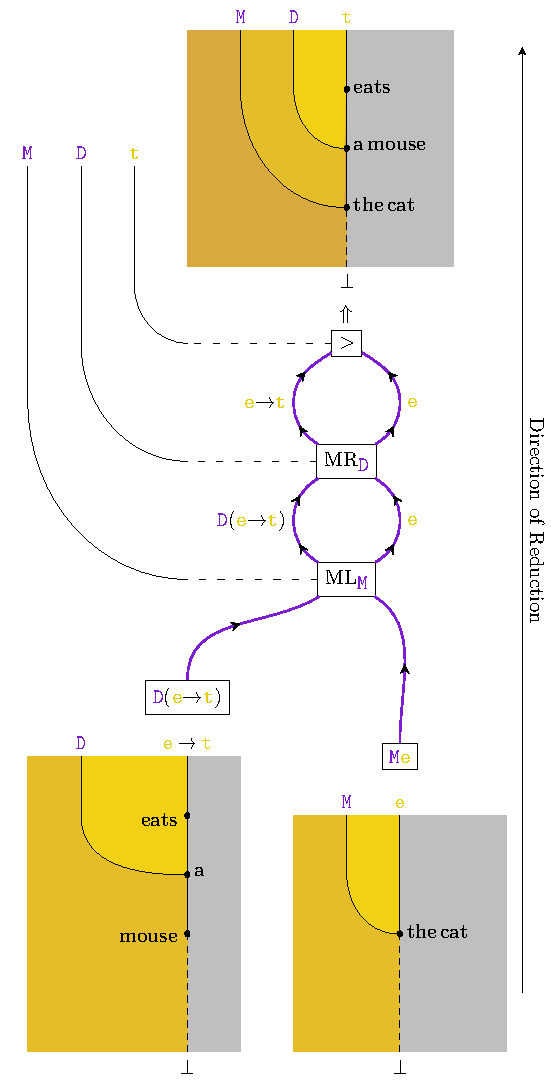
\includegraphics[width=.45\textwidth]{parsing-diagram}
	\caption{Representation of a parsing diagram for the sentence
		\emph{the cat eats a mouse}.
		See Figure \ref{fig:tree-box} for translation in a parse tree.}
	\label{fig:parsing-diagram}
\end{wrapfigure}

While we have gone with the hypothesis that we have a CFG for our language,
any type of polynomial-time structure could work, as long as it is more
expressive than a CFG.

The \emph{polynomial time combinators} assumption in the following theorem is
not a complex assumption, this is for example true for denotations based on
lambda-calculus, with function application being linear in the number of uses
of variables in the function term, which in turn is linear in the number of
terms used to construct the function term and thus of words, and the different
\fmap being in constant time for the same reason.

\begin{theorem}
	\label{thm:ptime-denot}
	Retrieving a pure denotation for a sentence can be done in polynomial time in
	the length of the sentence, given a polynomial time syntactic parsing
	algorithm and polynomial time combinators.
\end{theorem}

\begin{proof}
	We have proved in Theorem \ref{thm:ptime-parse} that we can retrieve a
	semantic parse tree from a	sentence in polynomial time in the input.
	Since we also have shown that the length of a semantic parse tree is quadratic
	in the length of the sentence it represents, being linear in the length of a
	syntactic parse tree linear in the length of the sentence.
	We have already seen that given a denotation, handling all effects and
	reducing effect handling to normal forms can be done in polynomial time.
	The superposition of these steps yields a polynomial-time algorithm in the
	length of the input sentence.
\end{proof}


\subsection{Diagrammatical Parsing}
\label{subsubsec:diagram-parsing}
When considering \cite{coeckeMathematicalFoundationsCompositional2010}
way of using string diagrams for syntactic parsing/reductions, we can see them
as (yet) another way of writing our parsing rules.
In our typed category, we can make see our combinators as natural
transformations ($2$-cells): then we can see the different sets of combinators
as different arity natural transformations.
$>$, $\combML_{\f{F}}$ and $\combJ_{\f{F}}$ are represented in
Figure \ref{fig:combinator-sd}, up to the coloring of the regions, because that
is purely for an artistic rendition.

\begin{figure}[t]
	\centering
	\begin{equation*}
	\begin{tikzpicture}[baseline={([yshift=-.5ex]current bounding box.center)}]
		\path coordinate[dot, label=below:$>$] (m)
		+ (0, 1) coordinate[label=above:$\beta$] (result)
		+ (-1, -1) coordinate[label=below:$\alpha \to \beta$] (phi)
		+ (1, -1) coordinate[label=below:$\alpha$] (x);
		\draw (m) -- (result);
		\draw (m) to[out=180, in=90] (phi);
		\draw (m) to[out=0, in=90] (x);
		\begin{pgfonlayer}{background}
			\fill[catmcb] (result) -- (m) -- ($(m) + (-1, 0)$) |- (result);
			\fill[catmcb] (result) -- (m) to[out=180, in=90] (phi) -- ($(phi) + (-1, 0)$) |- (result);
			\fill[catmc] (result) -- (m) -- ($(m) + (1, 0)$) |- (result);
			\fill[catmc] (result) -- (m) to[out=0, in=90] (x) -- ($(x) + (1, 0)$) |- (result);
			\fill[catmca] (m) to[out=0, in=90] (x) -- (phi) to[out=90, in=180] (m);
		\end{pgfonlayer}
	\end{tikzpicture}
	\hspace{2.5cm}
	\begin{tikzpicture}[baseline={([yshift=-.5ex]current bounding box.center)}, yscale=-1]
		\path coordinate[dot, label=above:$\combML_{\f{F}}$] (m)
		+ (1, 1) coordinate[label=below:$\beta$] (out2)
		+ (-1, 1) coordinate[label=below:$\alpha$] (out)
		+ (-1.5, 1) coordinate[label=below:$\f{F}$] (out1)
		+ (-1, -1) coordinate[label=above:$\alpha$] (phi)
		+ (1, -1) coordinate[label=above:$\beta$] (x);
		\draw (m) to[out=180, in=90] (phi);
		\draw (m) to[out=0, in=90] (x);
		\draw (m) to[out=180, in=-90] (out1);
		\draw (m) to[out=180, in=-90] (out);
		\draw (m) to[out=0, in=-90] (out2);
		\begin{pgfonlayer}{background}
			\fill[catmcc] (m) to[out=180, in=90] (phi) -- ($(phi) + (-1, 0)$) |- (out1) to[out=-90, in=180] (m);
			\fill[catmc] (m) to[out=0, in=-90] (x) -- ($(x) + (1, 0)$) |- (out2) to[out=-90, in=0] (m);
			\fill[catmca] (m) to[out=180, in=90] (phi) -- (x) to[out=90, in=0] (m);
			\fill[catmcb] (m) to[out=180, in=-90] (out1) -- (out) to[out=-90, in=180] (m);
			\fill[catmca] (m) to[out=180, in=-90] (out) -- (out2) to[out=-90, in=0] (m);
		\end{pgfonlayer}
	\end{tikzpicture}
	\hspace{2.5cm}
	\begin{tikzpicture}[baseline={([yshift=-.5ex]current bounding box.center)}]
		\path coordinate[dot, label=below:$\combJ_{\f{F}}$] (m)
		+ (0, 1) coordinate[label=above:$\f{F}$] (result)
		+ (-1, -1) coordinate[label=below:$\f{F}$] (phi)
		+ (1, -1) coordinate[label=below:$\f{F}$] (x);
		\draw (m) -- (result);
		\draw (m) to[out=180, in=90] (phi);
		\draw (m) to[out=0, in=90] (x);
		\begin{pgfonlayer}{background}
			\fill[catmcb] (result) -- (m) -- ($(m) + (-1, 0)$) |- (result);
			\fill[catmcb] (result) -- (m) to[out=180, in=90] (phi) -- ($(phi) + (-1, 0)$) |- (result);
			\fill[catmc] (result) -- (m) -- ($(m) + (1, 0)$) |- (result);
			\fill[catmc] (result) -- (m) to[out=0, in=90] (x) -- ($(x) + (1, 0)$) |- (result);
			\fill[catmca] (m) to[out=0, in=90] (x) -- (phi) to[out=90, in=180] (m);
		\end{pgfonlayer}
	\end{tikzpicture}
\end{equation*}

	\caption{String Diagrammatic Representation of Combinator Modes $>, \combML$ and $\combJ$}
	\label{fig:combinator-sd}
\end{figure}

Now, a way to see this would be to think of this as an orthogonal set of
diagrams to the ones of Section \ref{sec:nondet}: we could use the syntactic
version of the diagrams to model our parsing, according to the rules in
Figure \ref{fig:combination-cfg}, and then combine the diagrams as shown in
Figure \ref{fig:parsing-diagram}, which highlights why we can consider the
diagrams orthogonal.
In this figure we exactly see the sequence of reductions play out on the types
of the words, and thus we also see what exact \emph{quasi-braiding} would be
needed to construct the effect diagram.
Here we talk about \emph{quasi-braiding} because, in a sense, we use $2$-cells
to do braiding-like operations on the strings, and don't actually allow for
braiding inside the diagrammatic computation.
To better understand what happens in those parsing diagrams, Figure
\ref{fig:parsing-trees} provides the translations in labelled trees of the
parsing diagrams of Figures \ref{fig:parsing-diagram},
\ref{fig:parsing-diagram2} and \ref{fig:3dparsing-diagram}.

\begin{wrapfigure}{r}{.45\textwidth}
	\centering
	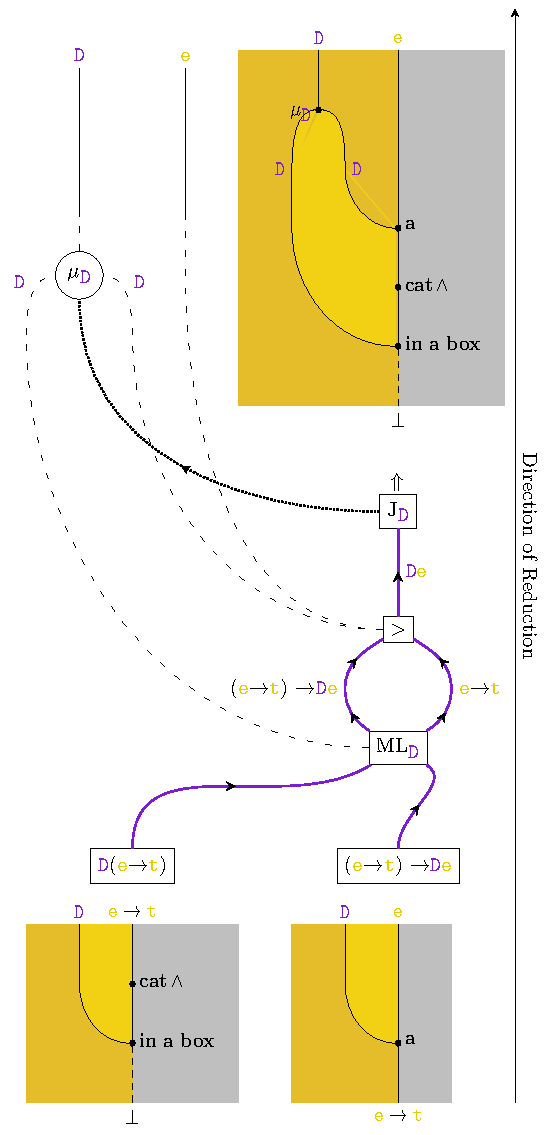
\includegraphics[width=.45\textwidth]{parsing-diagram2.pdf}
	\caption{Example of a parsing diagram for the phrase
		\emph{a cat in a box}, presenting the integration of unary combinators
		inside the connector line. See Figure \ref{fig:tree-box} for translation in
		a parse tree.}
	\label{fig:parsing-diagram2}
\end{wrapfigure}

Categorically, what this means is that we start from a meaning category $\mC$,
our typing category, and take it as our grammatical category.
This is a form of extension on the monoidal version by
\cite{coeckeMathematicalFoundationsCompositional2010}, as it is seemingly a
typed version, where we change the pregroup category for the typing category,
possibly taken with a product for representation of the English grammar
representation, to accommodate for syntactic typing on top of semantic typing.
This is, again, just another rewriting of our typing rules.


We have a first axis of string diagrams in the category
$\mC$ - our string diagrams for effect handling, as in Section
\ref{sec:nondet} - and a second \emph{orthogonal} axis of string diagrams
on a larger category, with endofunctors labelled
by the types in our typing category $\bar{\mC}$ and
with natural transformations mapping the combinators defined in Figures
\ref{fig:combination-cfg} and \ref{fig:combinator-denotations}.
The category in which we consider the second-axis string diagrams does not have
a meaning in our compositional semantics theory, and to be more precise, we
should talk about $1$-cells and $2$-cells instead of functors and natural
transformations, to keep in the idea that this is really just a diagrammatic
way of computing and presenting the operations that are put to work during
semantic parsing:
A good approach to these diagrams is that they are an extension of the
labelled parse trees presented in
\cite{bumfordEffectdrivenInterpretationFunctors2025}, forming a full
diagrammatic calculus system for semantic parsing.

\smallskip

For the combinators $\combJ$, $\combDN$ and $\combC$, which are applied to
reduce the number of effects inside a denotation, it might seem less obvious
how to include them.
Applying them to the actual \emph{parsing} part of the diagram is done
in the exact same way as in the CFG: we just add them where needed, and they
will appear in the resulting denotation as a form of forced handling, in a
sense, as shown in the result of Figure \ref{fig:parsing-diagram2}.

\begin{wrapfigure}[14]{r}{.45\textwidth}
	\centering
	\begin{tikzpicture}
		\node (fig) at (0, 0) {
\includegraphics[width=.4\textwidth]{knitting-example}};
		\draw[->] ($(fig.south west) + (-.1, -.1)$) -- node[anchor=east] {\rotatebox{90}{Direction of Reduction}} ($(fig.north west) + (-.1, .1)$);
	\end{tikzpicture}
	\caption{Example of a \emph{Jacquard} knitwork. Photography and work courtesy
		of the author's mother.}
	\label{fig:knitting-example}
\end{wrapfigure}

It is interesting to note that the resulting diagram representing
the sentence can visually be found in the connection strings that arise from
the combinators.
The main reason why this point of view of diagrammatic parsing is useful
will be clear when looking at the rewriting rules and the normal forms they
induce, because, as seen before, string diagrams make it easy to compute
normal forms, when provided with a confluent reduction system.

The other reason being the tangible interpretation of how things work
underlying the idea of a string diagram:
Suppose you're knitting a rainbow scarf.
You have multiple threads (the different words) of the different colours (their
types and effects) you're using to knit the scarf.

\begin{wrapfigure}[23]{l}{.5\textwidth}
	\centering
	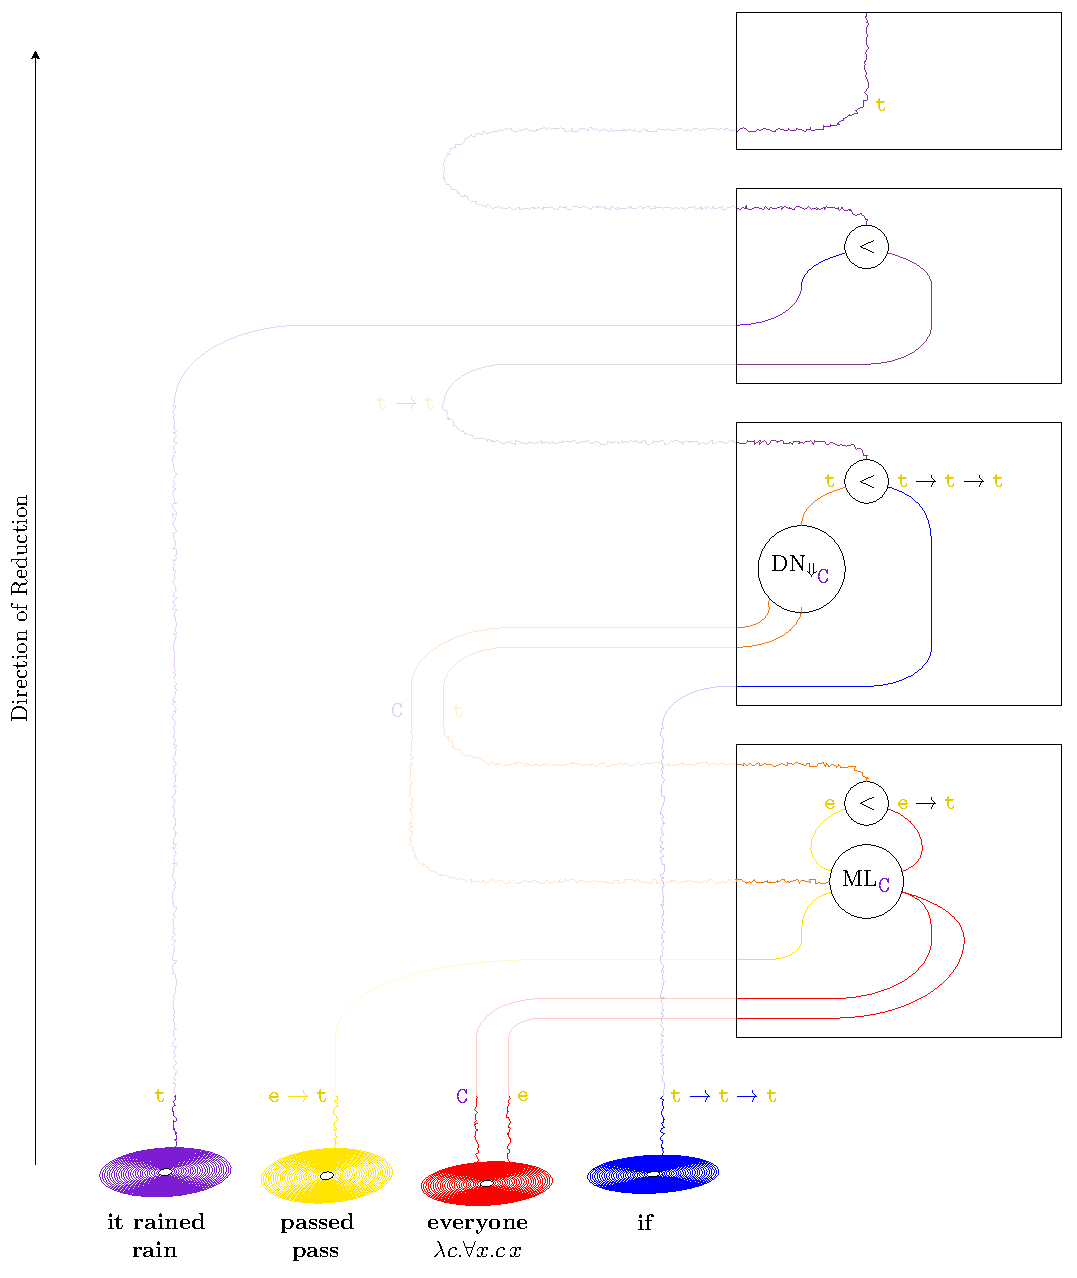
\includegraphics[width=.5\textwidth]{3d-parsing-diagram}
	\caption{Knitting-like representation of the diagrammatic parsing of a sentence. See Figure \ref{fig:tree-rain} for the translation in a parse tree}
	\label{fig:3dparsing-diagram}
\end{wrapfigure}

When you decide to change the color you take the different threads you have
been using, and mix them up.
You can create a new colour\footnote{This is not how wool works, but
	if one can also imagine a pointillist-like way of drawing using multiple
	coloured lines that superimpose on each other, or a marching band's multiple
	instruments playing either in harmony or in disharmony and changing that
	during a score.} thread from two (that's the base combinators) create a
thicker one from two of the same colour (the applicative mode and the monadic
join), put aside a thread until a later step (that's the $\fmap$), add a new
thread to the pattern (that's the unit), or cut a thread you will not be
using anymore (that's the co-units and closure operators).
Changing a thread by cutting it and making a knot at another point is basically
what the eject combinators do.
This more tangible representation can be seen in a larger diagram in Figure
\ref{fig:3dparsing-diagram}.



The sections in the rectangle represent what happen when considering our
combination step as implementing patterns inside a knitwork, as seen in Figure
\ref{fig:knitting-example}.
The different patterns provide, in order, a visual representation of the
different ways one can combine two strings, i.e., two types and thus two
denotations.
The sections outside of the rectangle are the strings of yarn not currently
being used to make a pattern.

\subsection{Rewriting Rules}
\label{subsec:rewrite}
Here we provide a rewriting system on that allows us to
improve our time complexity by reducing the size of the grammar.
In the worst case, in big o notation there is no improvement in the size of the
sentence, but there is no loss.

\smallskip

First consider the case where we have presuppositions (or sub-trees) for the
two arguments of our parsing step, that are of type $\f{F}\tau$ and
$\f{G}\tau'$.
In that case we could either get a result with effects $\f{F}\f{G}$ or
with effects $\f{G}\f{F}$ (or possibly more).
In general those effects are not the same, but if they happen to be, which
trivially will be the case when one of the effects is external (the plural or
islands functors for example), the order of application does not matter and
thus we choose to get the outer effect the one of the left side of the
combinator.

\smallskip

Then there are sequence of modes that clearly encompass other ones
the grammar notation for ease of explanation.
One should not use the unit of a functor after using $\combML$ or $\combMR$, as
that adds void semantics.
Same things can be said for certain other derivations containing the lowering
and co-unit combinators:

\noindent We use $\combDN$ when we have not used any of the following, in all
derivations:
\begin{multicols}{2}
	\begin{itemize}
		\item $m_{\f{F}}, \combDN, m_{\f{F}}$ where
		      $m \in \{\combMR, \combML\}$
		\item $\combML_{\f{F}}, \combDN, \combMR_{\f{F}}$
		\item $\combA_{\f{F}}, \combDN, \combMR_{\f{F}}$
		\item $\combML_{\f{F}}, \combDN, \combA_{\f{F}}$
		\item $\combC$
	\end{itemize}
\end{multicols}
\noindent We use $\combJ$ if we have not used any of the following,
for $j \in \{\epsilon, \combJ_{\f{F}}\}$
\begin{multicols}{2}
	\begin{itemize}
		\item $\left\{m_{\f{F}}, j, m_{\f{F}}\right\}$ where
		      $m \in \{\combMR, \combML\}$
		\item $\combML_{\f{F}}, j, \combMR_{\f{f}}$
		\item $\combA_{\f{F}}, j, \combMR_{\f{F}}$,
		\item $\combML_{\f{F}}, j, \combA_{\f{F}}$
		\item $k, \combC$ for $k \in \{\epsilon, \combA_{\f{F}}\}$
		\item If $\f{F}$ is commutative as a monad:
		      \begin{itemize}
			      \item $\combMR_{\f{F}}, \combA_{\f{F}}$
			      \item $\combA_{\f{F}}, \combML_{\f{F}}$
			      \item $\combMR_{\f{F}}, j, \combML_{\f{F}}$
			      \item $\combA_{\f{F}}, j, \combA_{\f{F}}$
		      \end{itemize}
	\end{itemize}
\end{multicols}

\begin{theorem}
	The rules proposed above yield equivalent results.
\end{theorem}
\begin{proof}
	For the first point, it is obvious since based on an equality.
	For the second point:
	The rules about not using combinators $\combUL$ and $\combUR$ come from the
	notion of handling and granting termination and decidability to our system.
	The rules about adding $\combJ$ and $\combDN$ after moving two of the same
	effect from the same side (i.e. $\combML \combML$ or $\combMR\combMR$) are
	normalization of Theorem \ref{thm:isotopy}.
	Indeed, in the denotation, the only reason to keep two of the same effects
	and not join them is to at some point	have something get in between the two.
	Joining and closure should then be done at earliest point in parsing where t
	can be done, and that is equivalent to later points because of the elevator
	equations, or Theorem \ref{thm:isotopy}.
	The last set of rules follows from the following: we should not use $\combJ
		\combML \combMR$ instead of $\combA$, as those are equivalent because of the
	equation defining them.
	The same thing goes for the other two, as we should use the units of monads
	over applicative rules and \fmap.
\end{proof}

When using our diagrammatic approach to parsing, we can write all the
reductions described above to our paradigm: it simply amounts to
constructing a set of equational reductions for the string diagrams.
This leads to the same algorithms developed in Section \ref{sec:nondet} being
usable here: we just have a new improved version of Theorem
\ref{thm:confluence} which adds the normal forms specified in this section to
the newly added \emph{orthogonal} axis of diagrammatic computations.
What we're actually doing is computing two different normal forms along the
tensor product of our reduction schemes, which amounts to computing a larger
normal form.
Moreover, considering the possible normal forms of syntactic reductions
or denotational reductions adds ways to reduce our diagrams to normal forms.
Of course, this does not mean that our system is complete, as there might still
be many possible reductions to be found, although this would not reduce the
complexity of the algorithm and is more of a thought experiment.




\section{Conclusion}
The functional programming approach developed in
\cite{bumfordEffectdrivenInterpretationFunctors2025} allows for increased
expressiveness in the choice of denotations, especially from a purely
theoretical point of view.
In this paper we have successfully prove that it is well-founded theoretically,
but also that it doesn't come at the cost of comprehensibility or efficiency.

Moreover, while our methods for implementing a type and effect system have been
applied to natural language semantics, it could be applied in any language with
purely compositional semantics.
Of course, there are still improvements that can be made, in particular around
the unorthodox use of effects to define what we have called higher-order
constructs and scope islands, but also in integrating the theory in more
complicated models of denotations, such as the ones learned through a neural
network for example.
In that case, it would suffice to understand what base combinators exist for
the model to implement the formalism we described.

\appendix
\bibliography{tdparse.bib}

\section{Presenting a Language}
In this appendix, we provide tables (\ref{fig:lexicon} and \ref{fig:functors}) describing the
modeling of a subset of the English language in our formalism.

\begin{figure}[H]
	\centering
	\begin{subfigure}{.9\textwidth}
		\centering
			\setcellgapes{2pt}
	\makegapedcells
	\begin{NiceTabular}{>{\bf}LLL}
		Expression & \rm Type & \lambda\text{-Term} \\
		\word{planet}{\e\to\t}{\lambda x. \w{planet} x}{common nouns}
		\word{carnivorous}{\left( \e \to \t \right)}{\lambda x. \w{carnivorous}x}{predicative adjectives}
		\word{skillful}{\left( \e \to \t \right) \to \left( \e \to \t \right)}{\lambda p. \lambda x. px \land \w{skillful} x}{predicate modifier adjectives}
		\word{Jupiter}{\e}{{\bf j}\in \Var}{proper nouns}
		\word{sleep}{\e \to \t}{\lambda x. \w{sleep} x}{intranitive verbs}
		\word{chase}{\e \to \e \to \t}{\lambda o. \lambda s. \mathbf{chase}\left( o \right)\left( s \right)}{transitive verbs}
		\word{be}{\left( \e \to \t \right) \to \e \to \t}{\lambda p. \lambda x. px}{}
		\word{she}{\e\to\e}{\lambda x. x}{}
		\word{it}{\left( \bot \to \f{G}\e \right)}{\lambda g. g_{0}}{}
		\word{which}{\left( \e \to \t \right)\to \f{S}\e}{\lambda p. \left\{x \suchthat px\right\}}{}
		\word{the}{\left( \e \to \t \right) \to \f{M}\e}{\lambda p. x \text{ if } p^{-1}\left( \top \right) = \{x\} \text{ else } \#}{}
		\word{a}{\left( \e \to \t \right) \to \f{D}\e}{\lambda p. \lambda s. \left\{ \scalar{x, x + s}\suchthat p x\right\}}{}
		\word{no}{\left( \e \to \t \right) \to \f{C}\e}{\lambda p. \lambda c. \lnot \exists x. p x \land c\, x}{}
		\word{every}{\left( \e \to \t \right)\to \f{C}\e}{\lambda p. \lambda c. \forall x, px \Rightarrow cx}{}
		\CodeAfter
		\begin{tikzpicture}
			\draw[double] (1|-2) -- (4|-2);
			\foreach \r in {4,6,...,14} {\draw (1|-\r) -- (4|-\r);}
			\foreach \r in {15,...,21} {\draw (1|-\r) -- (4|-\r);}
		\end{tikzpicture}
	\end{NiceTabular}

		\caption{Lexicon for a subset of the English language}
		\label{fig:lexicon}
	\end{subfigure}

	\medskip

	\begin{subfigure}{\textwidth}
		\centering
		\resizebox{\textwidth}{!}{%
				\def\arraystretch{1.3}
	\setcellgapes{2pt}
	\makegapedcells
	\begin{NiceTabular}{LLc}
		\rm Constructor                                              & \fmap                                                                                     & Typeclass \\
		\f{G}\left( \tau \right) = \r \to \tau                       & \f{G}\phi\left( x \right) = \lambda r. \phi \left(x r\right)                              & Monad     \\
		\f{W}\left( \tau \right) = \tau \times \t                    & \f{W}\phi\left( \left( a, p \right) \right) = \left( \phi a, p \right)                    & Monad     \\
		\f{S}\left( \tau \right) = \{ \tau \}                        & \f{S}\phi\left( \left\{ x \right\} \right) = \left\{ \phi(x) \right\}                     & Monad     \\
		\f{C}\left( \tau \right) = \left( \tau \to \t \right) \to \t & \f{C}\phi\left( x \right) = \lambda c. x\left( \lambda a. c \left( \phi a \right) \right) & Monad     \\
		\f{M}\left( \tau \right) = \tau + \bot                       & \f{M}\phi\left( x \right) = \begin{cases}
			                                                                                           \phi\left( x \right) & \text{if } \cont x: \tau \\
			                                                                                           \#                   & \text{if } \cont x: \#
		                                                                                           \end{cases}                                        & Monad                \\
		\CodeAfter
		\begin{tikzpicture}
			\draw[double] (1|-2) -- (5|-2);
			\foreach\r in {3,...,6} {%
					\draw (1|-\r) -- (5|-\r);
				}
		\end{tikzpicture}
	\end{NiceTabular}

		}
		\caption{Definition of a few functors, with their map on functions}
		\label{fig:functors}
	\end{subfigure}
	\caption{Presentation of a lambda-calculus lexicon for the English language}
\end{figure}


\end{document}
